%%%%%%%%%%%%%%%%%%%%%%%%%%%%%%%%%%%%%%%%%
% Beamer Presentation
% LaTeX Template
% Version 1.0 (10/11/12)
%
% This template has been downloaded from:
% http://www.LaTeXTemplates.com
%
% License:
% CC BY-NC-SA 3.0 (http://creativecommons.org/licenses/by-nc-sa/3.0/)
%
%%%%%%%%%%%%%%%%%%%%%%%%%%%%%%%%%%%%%%%%%

%----------------------------------------------------------------------------------------
%	PACKAGES AND THEMES
%---------------------------------------------------------------------------------------

\documentclass{beamer}
\usepackage[spanish]{babel}
 \usepackage{algpseudocode}
\usepackage[utf8]{inputenc}
\mode<presentation> {


\usetheme{PaloAlto}

}

\usepackage{graphicx} % Allows including images


%----------------------------------------------------------------------------------------
%	TITLE PAGE
%----------------------------------------------------------------------------------------

\title[Práctica 4]{TSP} % The short title appears at the bottom of every slide, the full title is only on the title page

\author{Algorítmica} % Your name
\institute[UGR] % Your institution as it will appear on the bottom of every slide, may be shorthand to save space
{
Universidad de Granada \\ % Your institution for the title page
\medskip

}
\date{\today} % Date, can be changed to a custom date

\begin{document}

\begin{frame}
\titlepage % Print the title page as the first slide
\end{frame}

\begin{frame}
\frametitle{Índice} % Table of contents slide, comment this block out to remove it
\tableofcontents % Throughout your presentation, if you choose to use \section{} and \subsection{} commands, these will automatically be printed on this slide as an overview of your presentation
\end{frame}

%----------------------------------------------------------------------------------------
%	PRESENTATION SLIDES
%----------------------------------------------------------------------------------------

\section{Introducción }
\begin{frame}
	\frametitle{Introducción}
	\begin{itemize}
		\item El objetivo de esta práctica es resolver el problema del TSP utilizando para ello un enfoque Branch and Bound y, alternativamente, otro con Backtracking y comparar ambos.
	\end{itemize}
\end{frame}


%------------------------------------------------
\section{Ejercicio} 
\begin{frame}
	\frametitle{Enunciado del ejercicio}
	Se desea sentar a N invitados alrededor de una mesa, de manera que cada invitado tendrá a su lado a otros dos. Cada par de invitados tiene un nivel de compatibilidad. Se desea maximizar la compatibilidad de estos comensales.
	
\end{frame}

%------------------------------------------------
\section{Diseño del algoritmo: Branch and Bound} 
\begin{frame}
	\frametitle{Diseño del algoritmo}
		
		Usaremos una cola con prioridad que será donde se introduzcan los nodos.
		En la cola se seleccionará el nodo con mayor prioridad, y de dicho nodo se consultará el valor de su cota local, que en caso de ser mejor a la global se añadiran los hijos del nodo a la cola, y en caso de ser peor, se devuelve la solucion actual
	    
		
\end{frame}




\section{Pseudocódigo}

\begin{frame}
		\frametitle{Pseudocódigo}
		\footnotesize{	
		\begin{algorithmic}				
			\Require Matriz\_costes, Vector\_ciudades[N] Vector\_distancias\_minimas; 
			\State \textbf{Branch\&Bound( Matriz\_costes, Vector\_ciudades Vector\_distancias\_minimas):}
				\State priority\_queue cola;
				\State Ciudades\_Visitadas[N,FALSE];
				\State solucion\_parcial,solucion\_final;
				\State	 Nodo n.generarnodo(Vector\_ciudades[0])
			\While {\textbf{!cola.empty()}{
					nodo = cola.top();
					\If(nodo.cotalocal > cota global ){
						return solucion\_actual
					\Endif
					\Else{
						cola.add(nodo.generarhijos())
					}
					\Endelse
					
					}
				
			\EndWhile
	
			
				
				
			\end{algorithmic}	
		
\end{frame}

\section{Eficiencia}


\begin{frame}
	\frametitle{Eficiencia Empírica}	
	
	\begin{figure}[H]
		\centering
		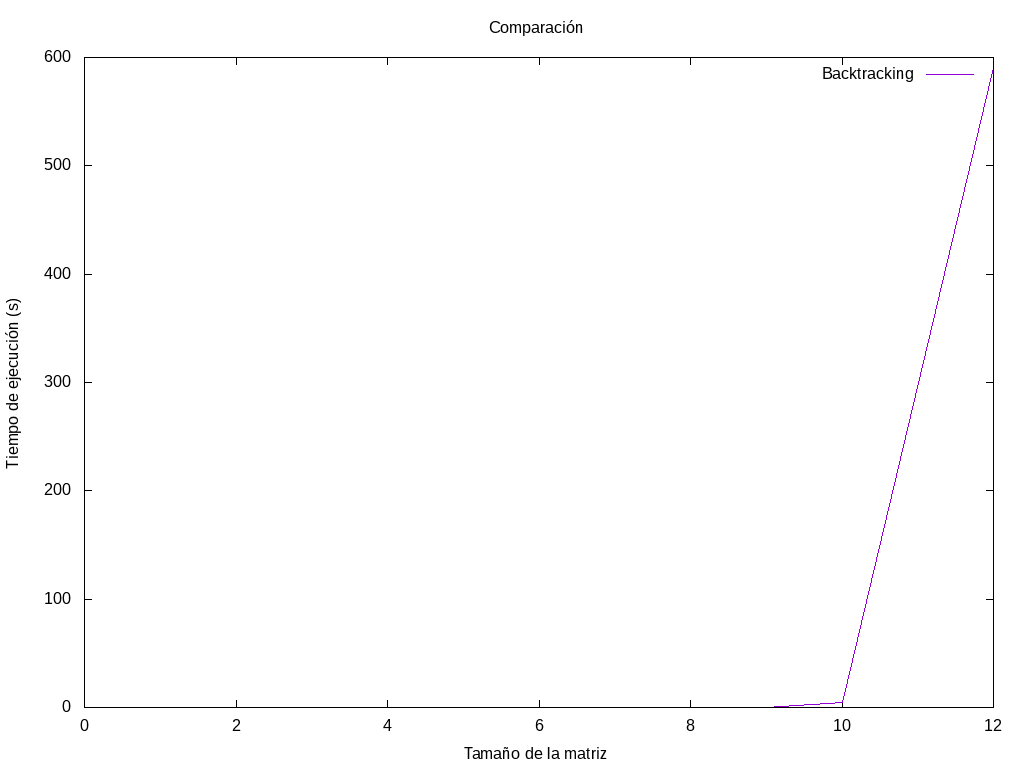
\includegraphics[width=0.7\linewidth,scale=1.5]{../Codigo/backtrackempirica}
		\caption{algoritmo backtracking}
		\label{fig:backtrackhibrida}
	\end{figure}
	
	
	
\end{frame}







\begin{frame}
	\frametitle{Eficiencia Híbrida}	

		\begin{figure}[H]
\centering
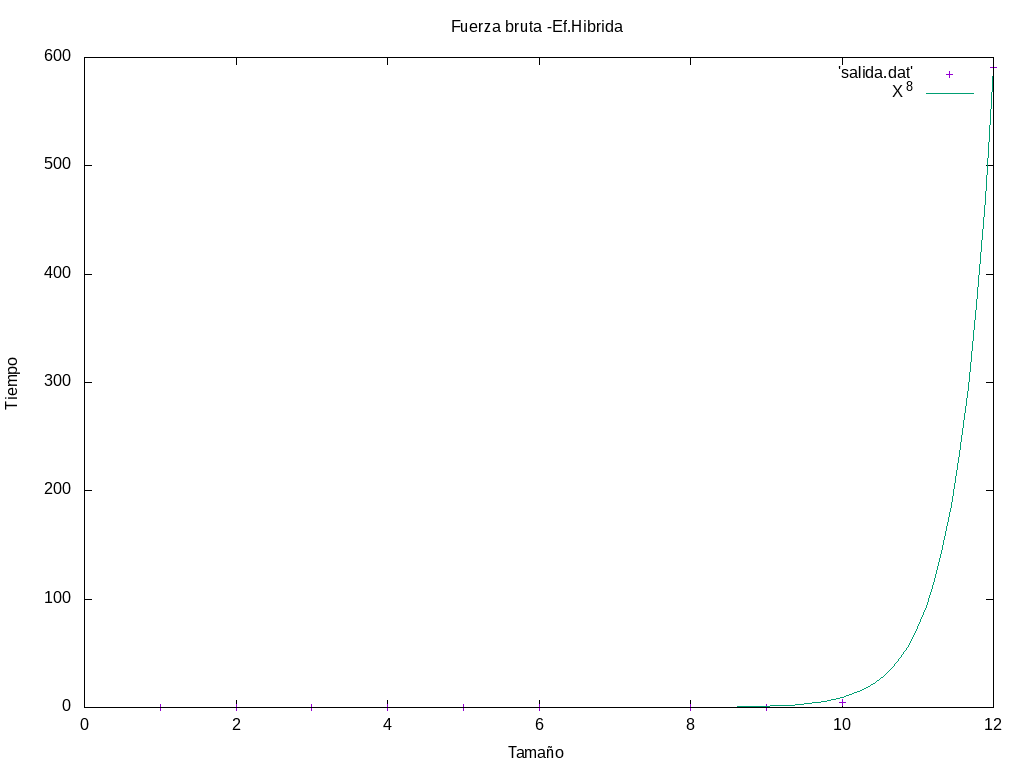
\includegraphics[width=0.7\linewidth,scale=1.5]{../Codigo/backtrackhibrida}
\caption{comparación x**8 vs algoritmo backtracking}
\label{fig:backtrackhibrida}
\end{figure}


	
\end{frame}

\begin{frame}
	\frametitle{Eficiencia Híbrida}	
	Ajuste con X**8

	\begin{table}[]
		\centering
		\caption{Ef híbrida obtenida}
		\label{my-label}
		\begin{tabular}{lllll}
			& Final set of parameters &   Asymptotic Standard Error & \\
			& a0  = 8.59555e-09 &  +/- 2.326e-11    (0.2706\%)&  \\
		
		\end{tabular}
	\end{table}
	
	
	
\end{frame}



\end{document} 
